\chapter{Implementation and Methodology}
\label{ch:experimental}
After review of the background of near-Earth asteroid surveys and the existing body of literature for modelling surveys, this chapter will discuss the developed simulation in more detail. Firstly, in \autoref{sec:methodologysimulation}, the architecture of the simulation is discussed on a top-level. Then, in \autoref{sec:methodologyimplementation}, the implementation of the components of the simulation based on the literature in \autoref{ch:surveymodelling} is explained. Then, discourse will be given to the methods of optimization utilized in the research in \autoref{sec:methodologyoptimization}. Lastly, in \autoref{sec:methodologyprocess}, the process of using the simulation and optimization methods to obtain the results and conclusions presented in the next chapter is explained as well as the reasoning to support the optimization results. For reference, the interested reader can find the complete code as-is \href{https://github.com/ArjanVermeulen97/thesis-code.git}{on Github} (\cite{GitHub}).

\section{Simulation Overview}
\label{sec:methodologysimulation}
First, before discussing the specifics of implementation, a general overview of the simulation is given. The objective of the simulation is to accurately predict the performance of a NEA survey by a given system of spacecraft, on a given population of NEAs. Obtaining results, performing optimization, as well as performing verification and validation are not considered a part of the simulation, but rather a system utilizing it. The process of performing those steps will be further explained in \autoref{sec:methodologyprocess}.\\

\begin{figure}[htbp]
 \centering
 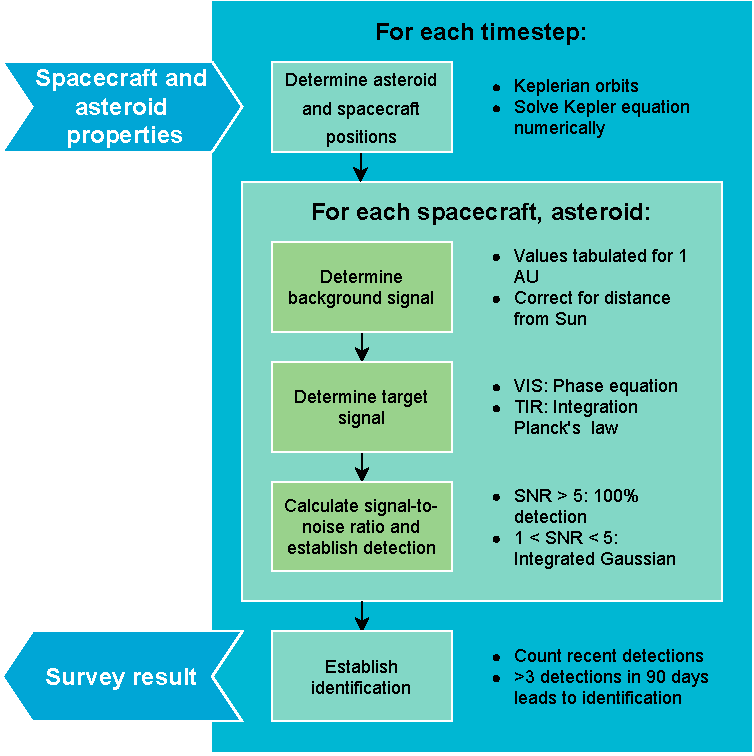
\includegraphics[width=0.7\textwidth]{img/simulation_overview.pdf}
 \caption{Overview of the simulation architecture and main loops.}
 \label{fig:simulation_overview}
\end{figure}

The architecture of the simulation is shown in \autoref{fig:simulation_overview}. On the top left, the main input parameters to the model are displayed. These are primarily the spacecraft and asteroid properties. Both of these consist of a full set of Keplerian orbital elements per spacecraft or asteroid. The asteroid properties furthermore include the albedo, size, and absolute magnitude of each asteroid; the spacecraft properties include which type of payload the spacecraft is carrying. \\

The simulation consists of a nested loop. Firstly, at the start of each timestep (the period between the timesteps is determined by the survey cadence), the positions of all asteroids and spacecraft are determined by propagation of their orbital elements using Keplerian orbital mechanics. Then, in the inside loop, each spacecraft is checked against each asteroid to see if that spacecraft can detect that asteroid. This is done through calculation of the signal-to-noise ratio (SNR). Lastly, as it is known which asteroids got succesfully detected by which spacecraft, it can be determined if asteroids have been identified. At the end of the simulation, the result is a list of the asteroid population in addition to whether they have been detected, and if so, when. Of course, this data can be further processed.

\section{Implementation}
\label{sec:methodologyimplementation}
In this section, the implementation of the simulation algorithm is discussed. The simulation was written fully in Python 3.8, for reasons of easy testing and iteration, availability of packages for data handling and analysis, and familiarity of the author. The simulations were ran on several computers equipped with consumer-grade 6-core CPU's. \\

With regards to specific packages, data handling and computation was performed using \href{https://pandas.pydata.org}{Pandas} and \href{https://numpy.org}{NumPy}. Where applicable, random seed values were fixed to the arbitrarily chosen value of 9. Parallelization was performed using \href{https://dask.org}{Dask}. Critical paths of these packages are written in C/C++/Cython, vastly improving the performance of the simulation. Optimization was implemented through \href{https://pypi.org/project/scikit-optimize}{Scikit-optimize} and \href{https://scikit-learn.org/stable/index.html}{Scikit-learn}. Where necessary for the purpose of analysis, data visualisation was performed using \href{https://seaborn.pydata.org}{Seaborn}. Several other packages were used, but their exact functionality and specification is not relevant for the implementation and operation of the simulation.

\subsection{Population of Asteroids, Spacecraft, and Orbital Mechanics}
The population of asteroids was implemented based on the work of \cite{GranvikPopulation}. The authors \href{http://www.iki.fi/mgranvik/data/Granvik+\_2018\_Icarus}{provide an already generated population model} of 802,000 NEAs of absolute magnitude $17 < H < 25$. This means that the generation and validation of the model does not need to be performed in this work. For the simulation, a random sample of asteroids is drawn for each simulation run. It was found that a number of 1000 asteroids provided adequate accuracy while reducing computational load. For validation runs, 2500 asteroids were sampled instead to ensure a higher level of accuracy.  The population data is implemented as a Pandas dataframe. Similarly, the spacecraft are also implemented as a Pandas dataframe, although their orbital elements and payload are given as input arguments to the simulation. \\

Orbits of asteroids and spacecraft were modelled using elliptical Keplerian orbits around the Sun, neglecting the gravitational influence of the Planets and other perturbations. As no complex mission gemetries or three-body interactions such as impacts are being studied, it was assumed that this would provide an accurate representation. MJD2000 is taken as epoch, and all simulations are run starting at that epoch. It is assumed that due to the even distribution of NEAs, this will not adversely affect the results (this is validated in \autoref{sec:vvsurvey}). The transcendental Kepler equation was solved numerically using the iterative method proposed by \cite{KeplerEquation}. As the eccentric anomaly is thus obtained directly from the mean anomaly, no numerical integration or propagation of the orbit is required. The resulting orbits and transformations were verified manually, the results of which can be found in \autoref{sec:vvsurvey}. It is noted that calculation of the position of asteroids and spacecraft, especially solving of the Kepler equation, presents one of the largest contributors to the simulation's runtime. For future work, an alternative implementation is recommended.

\subsection{Background Signal}
Implementation of the background signal as described in \autoref{sec:modelling_background} was carried out as follows: Data for visual light is directly provided in the work of \cite{LightOfTheNightSky} in tabulated format for a longitude range of $[0^\circ, 360^\circ]$, in intervals of $10^\circ$. Latitude coordinates are provided in the interval $[-90^\circ, 90^\circ]$, in intervals of $10^\circ$. Additionally, latitude values of $-15^\circ, -5^\circ, -2^\circ, 2^\circ, 5^\circ, 15^\circ$ are provided for improved detail around the brightest areas (such as the galactic core or the Sun). Background signal originating from the Sun is specified in the body-fixed frame relative to the Sun, $b$; signal from the background stars is specified in the galactic reference frame $g$. (Please refer to \autoref{sec:modelling_background} for a description of the reference frames). After manual verification, the tables were saved. \\

The thermal infrared signal as described in \cite{IRDust} was implemented in two steps. Firstly, the thermal infrared background signal from outside the Solar system was loaded, and the model for interplanetary dust and sunlight for the Sun-dependent portion of the background signal was implemented. For the latter, the required line-of-sight integration was performed numerically using a Riemann sum with a step size of 0.1 AU, up to a distance of 5.2 AU from the Sun. Results were verified manually by inspection, and comparison of coordinates of well-known objects in the Milky Way to their locations in the background star signal (see \autoref{sec:vvinfrared}). The latter step was taken to also ensure that the transformation from ecliptic to galactic coordinates was performed correctly. After verification, the resulting data was tabulated for the same longitude and latitude combinations as the visual light background signal. This was done to ensure universal operation of the code, reducing errors, and to avoid the computational load associated with processing the highly detailed \textit{COBE} data and performing the abovementioned numerical integration. \\

After tabulation, the background signal data can be stored fully in memory during operation. Where necessary, it can be corrected to account for the spacecraft's distance from the Sun using \autoref{eq:sunscale}. When necessary, the value of the signal is determined from interpolation by means of Scikit's linear N-dimensional interpolator. \autoref{fig:combinedvisbackground} and \autoref{fig:combinedtirbackground} show the resulting background signal in the visual light and thermal infrared, respectively. It can be seen, by comparing \autoref{fig:combinedtirbackground} to \autoref{fig:starstirbackground}, that some loss of detail in the thermal infrared is incurred due to the tabulation - this can be primarily observed through the loss of fidelity in small-scale structures in the fainter parts of the Milky Way - however the effect is minor.

\begin{figure}[htbp]
 \centering
 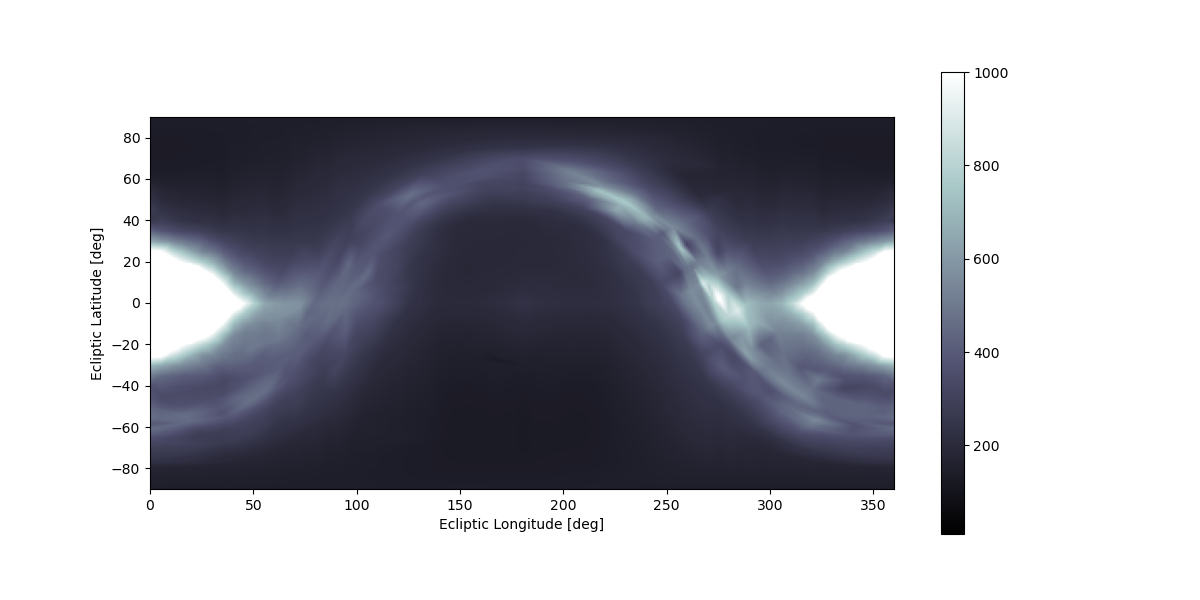
\includegraphics[width=1.0\textwidth]{img/background_vis_combined.png}
 \caption{Background signal in the visual spectrum, in the body-fixed reference frame $b$, as seen from a spacecraft located at (-1, 0, 0) AU in the heliocentric frame $h$. Units are $S10_\odot$ or solar-type stars of 10th magnitude per square degree. $1S10_\odot = 9.00\mathrm{W}\mathrm{m}^{-2}\mathrm{sr}^{-1}$. The scale is clipped at $1000 S10_\odot$ for clarity.}
 \label{fig:combinedvisbackground}
\end{figure}

\begin{figure}[htbp]
 \centering
 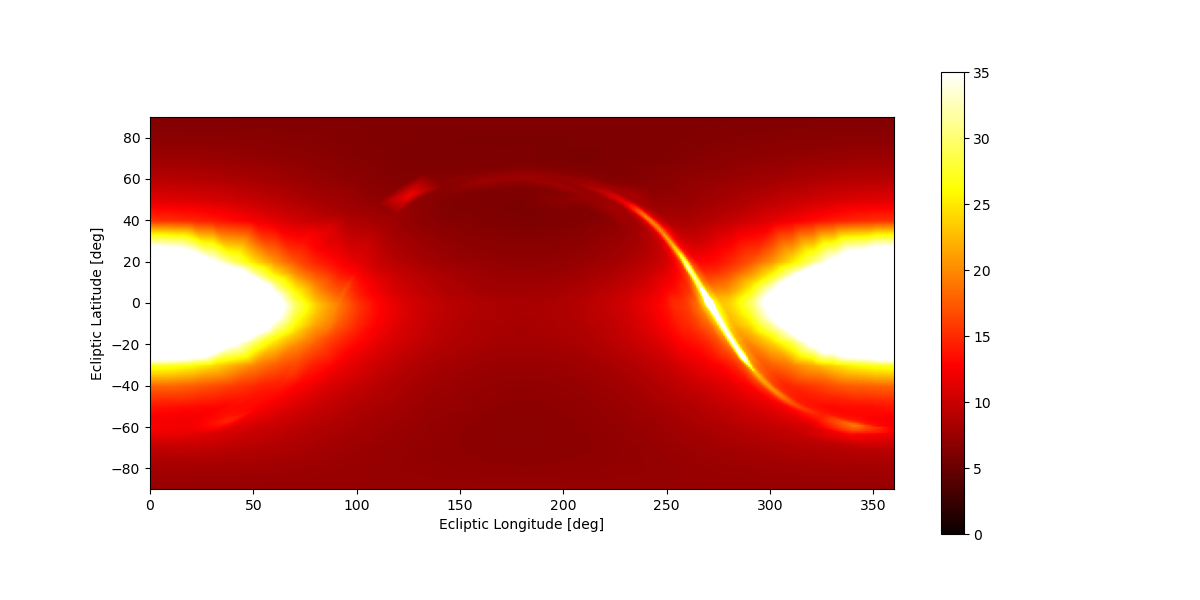
\includegraphics[width=1.0\textwidth]{img/background_tir_combined.png}
 \caption{Background signal in thermal infrared, in ecliptic coordinates, in the body-fixed reference frame $b$, as seen from a spacecraft located at (-1, 0, 0) AU in the heliocentric frame $h$. Units are Megajansky per steradian, $1 \mathrm{MJy}{sr}^{-1} = 10^{-21} \mathrm{W}\mathrm{m}^{-2}\mathrm{Hz}^{-1}\mathrm{sr}^{-1}$, and the scale is clipped at $35 \mathrm{MJy}{sr}^{-1}$ for clarity.}
 \label{fig:combinedtirbackground}
\end{figure}

\subsection{Target Signal}
Implementation of target signal is a straightforward process. For the visual spectrum, the formulae listed in \autoref{sec:modelling_target} could be directly copied. The thermal infrared signal involves a triple integration, and is slightly more complex. As this process has to be performed once for every combination of spacecraft and asteroid, at every timestep, performance has to be taken into account when implementing the integrations. \\

Firstly, the integration of Planck's law over the bandpass. No closed-form solution exists for the definite integral of Planck's law. As Planck's law is relatively smooth, the decision was made to approximate the integral by the average of the start and end of the bandpass. In practice this means:
\begin{equation}
 \int _{6 \mu\mathrm{m}}^{10 \mu\mathrm{m}} B(\lambda, T) d\lambda \approx \frac{1}{2}\left[B(6 \mu\mathrm{m}, T) + B(10 \mu\mathrm{m}, T)\right] \Delta \lambda
\end{equation}
This essentially approximates Planck's law as a linear function in the domain. It is assumed that this is accurate for the range and temperatures considered. This simplification has to be made, as this integration has to be carried out for every part of the numerical integration over the visible hemisphere of the asteroid, and is thus performed even more often per simulation - in fact, it is the most-called function in the simulation. The integration over the visual hemisphere of the asteroid is performed by first assuming the asteroid to be a sphere. From geometry this integral is well known:
\begin{equation}
 F(x) = \frac{D^2}{4}\int_{-\pi/2}^{\pi/2}\int_{-\pi/2}^{\pi/2} f(x) \cos \theta \cos \phi d \theta d \phi
\end{equation}
This integration was implemented through a Riemann sum as well, using the midpoint rule and an interval of $\pi/4$ for both directions, resulting in a total of 16 evaluations. It was found that the error with respect to a very precise integration was less than 1\%. Examples of the signal resulting from the implementation can be seen in \autoref{fig:visual_signal_implementation} for the visual wavelengths and \autoref{fig:thermal_signal_implementation} for the thermal infrared spectrum.

\begin{figure}[htbp]
 \centering
 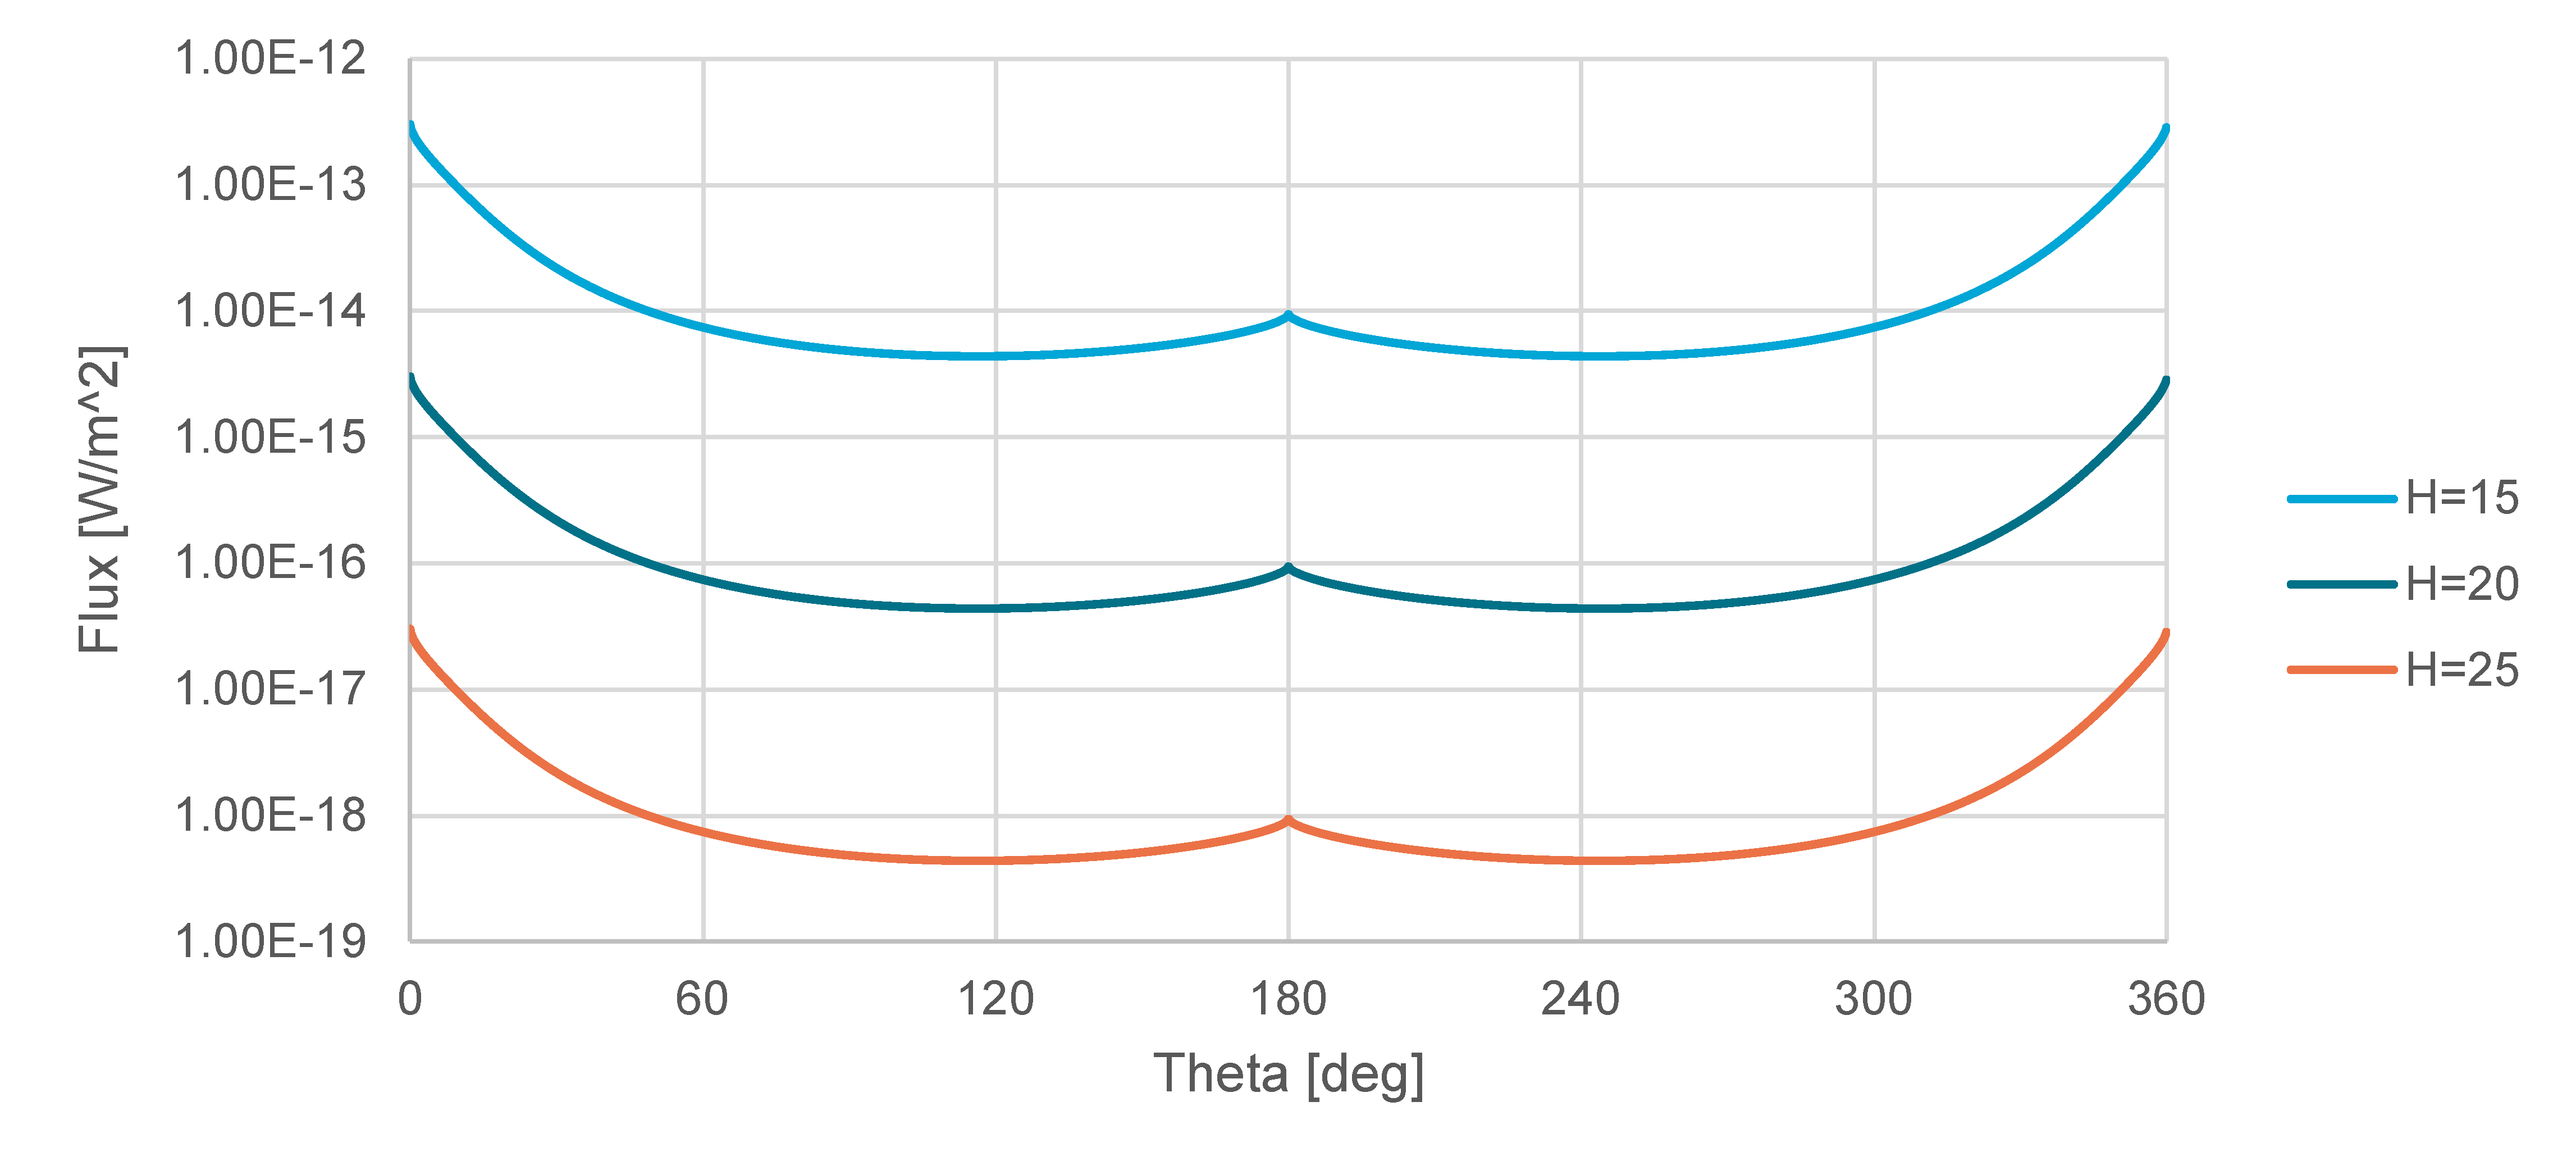
\includegraphics[width=0.8\textwidth]{img/implementation_vis_signal.pdf}
 \caption{Signal in the visual light spectrum of a $H=15, 20, 25; p_v=0.14$ asteroid in a 1 AU circular orbit around the Sun at zero inclination as seen from a spacecraft at (0.7, 0, 0) AU in the heliocentric frame $h$, as a function of the asteroid's true anomaly.}
 \label{fig:visual_signal_implementation}
\end{figure}


\begin{figure}[htbp]
 \centering
 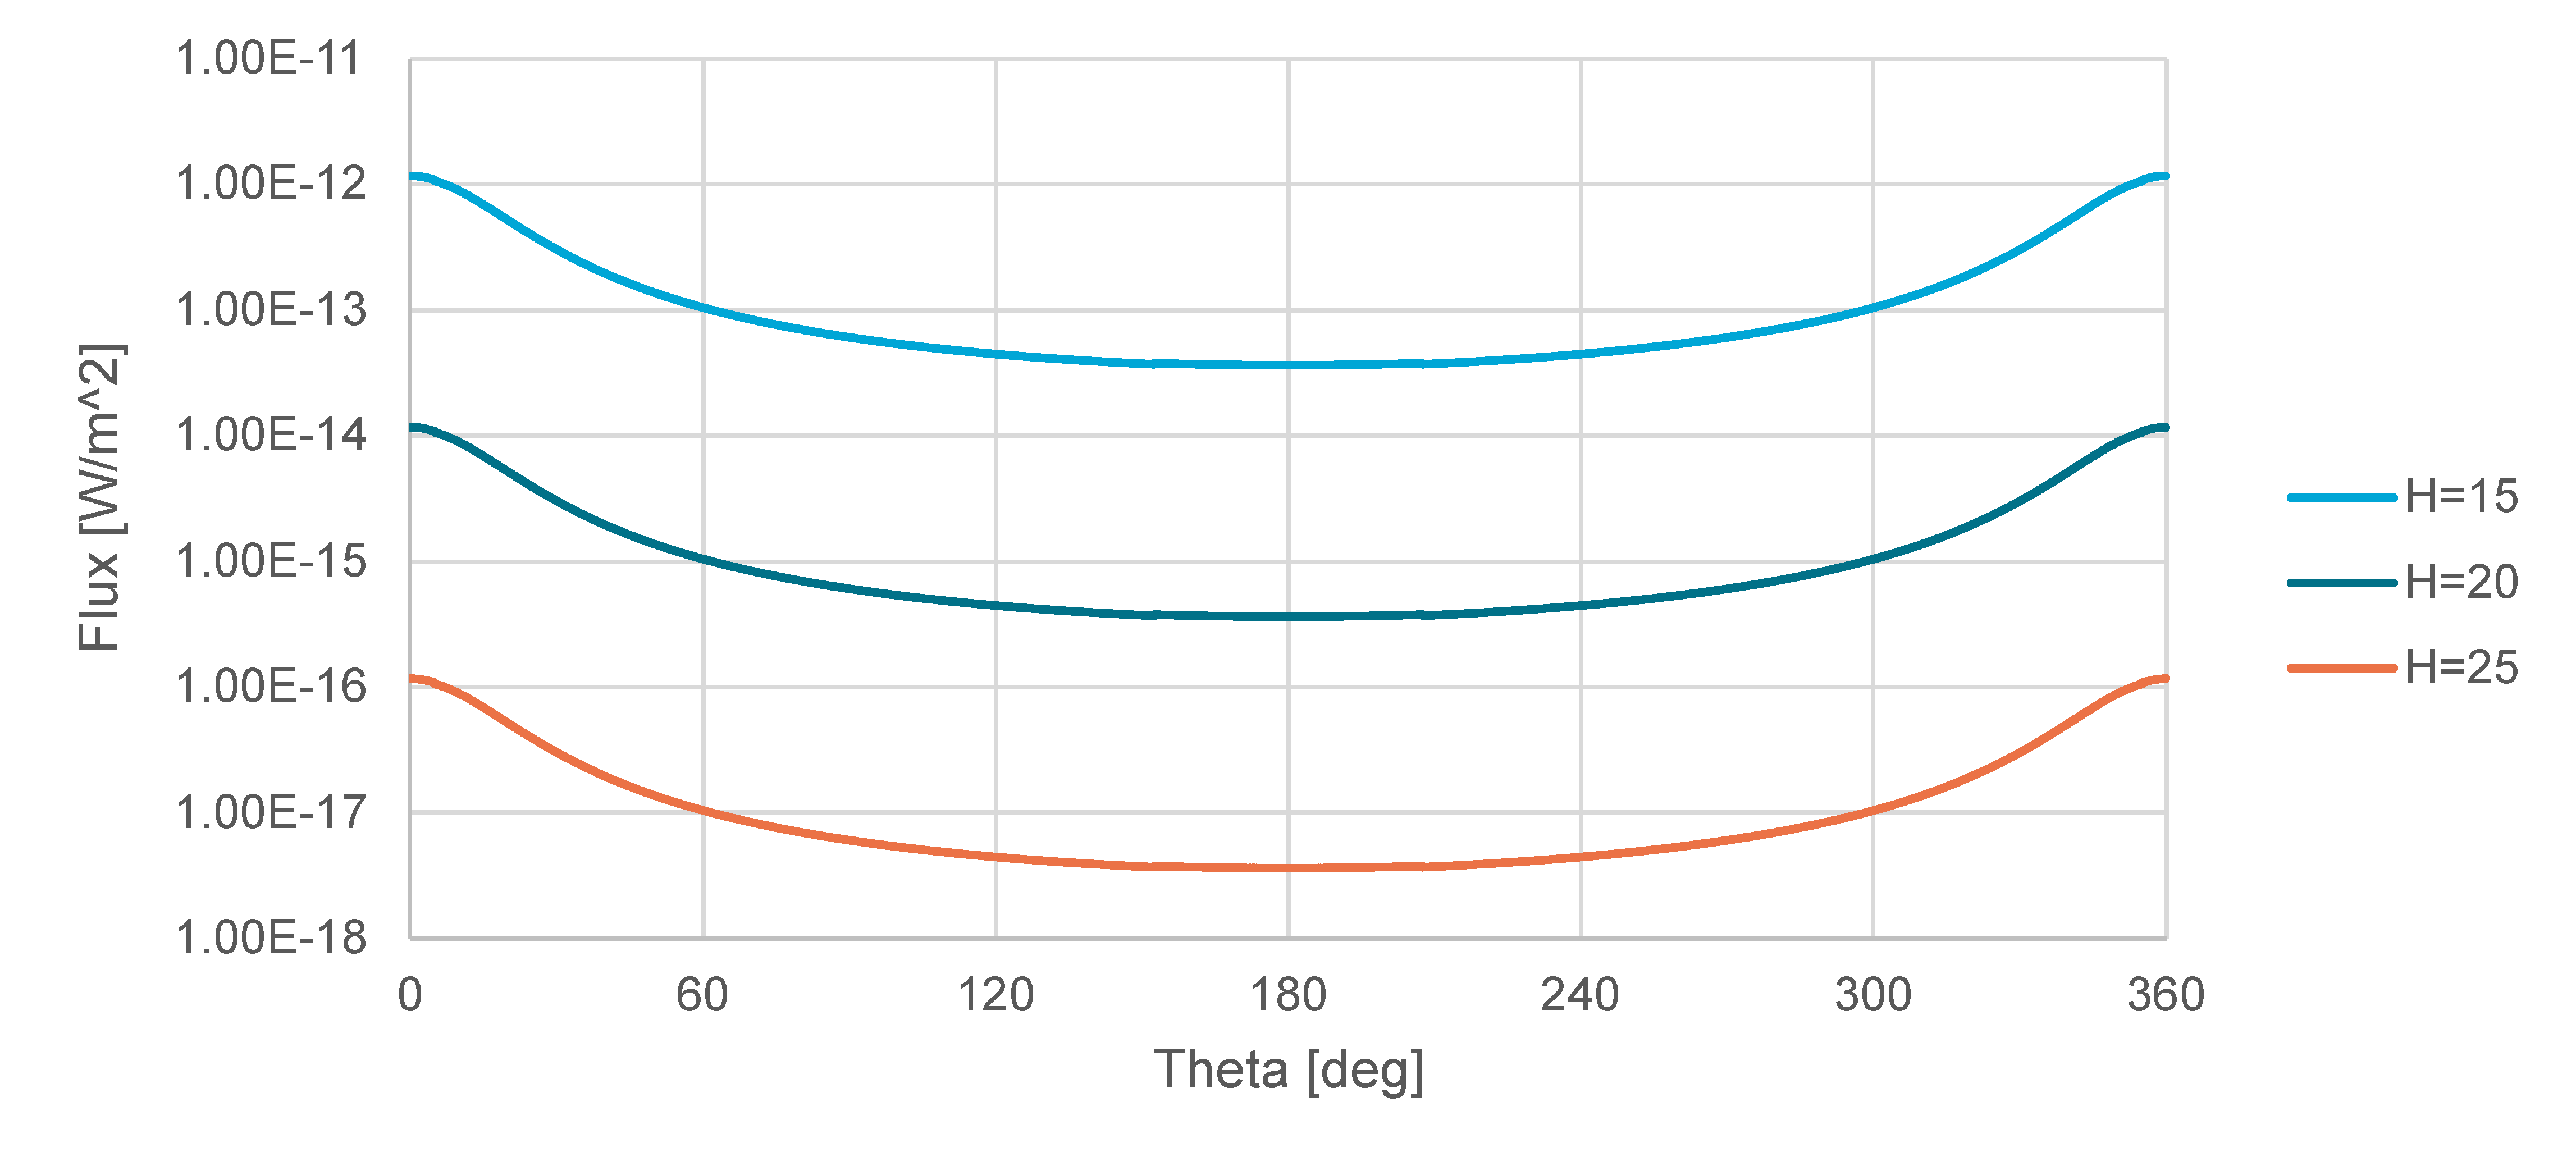
\includegraphics[width=0.8\textwidth]{img/implementation_tir_signal.pdf}
 \caption{Signal in the thermal infrared spectrum of a $H=15, 20, 25; p_v=0.14$ asteroid in a 1 AU circular orbit around the Sun at zero inclination as seen from a spacecraft at (0.7, 0, 0) AU in the heliocentric frame $h$ as a function of the asteroid's true anomaly.}
 \label{fig:thermal_signal_implementation}
\end{figure}

\subsection{Search Strategy and Cadence}
Implementation of the search strategy and cadence proved to be the most problematic aspect in the implementation process. As mentioned in \autoref{sec:modelling_cadence}, very little literature exists on the topic, and no methods have been developed to obtain an optimal search strategy utilizing multiple spacecraft. Several options were considered to model the strategy and resulting cadence. Firstly, a method omitting implementation, instead performing a correction ex post, such as utlized by \cite{ThesisOlga}. This method was expected to underrepresent the effect of a distinct survey cadence, and introduces a look-ahead bias which would both be very problematic for the accuracy of the results of this simulation. Secondly, explicitly modelling a north-to-south, west-to-east gridsearch-like strategy such as described by \cite{NEOCam} was considered. Although this model would arguably be the most accurate, it is very impactful with respect to the computational load, for three reasons:
\begin{itemize}
 \item Firstly, the positions of the asteroids and spacecraft have to be calculated for each imaging step. This results in calculating the positions $n_{images} = (360^2/\pi) / \Theta = 41,253~\mathrm{deg}^2 / (7.13^\circ*1.7^\circ) \approx 3400$ times for thermal infrared, or 734 times for the visual spectrum, for each complete scan of the sky (see \autoref{sec:modelling_cadence} for a more expansive description of this calculation).
 \item Secondly, to check whether or not an asteroid is inside the field-of-view of the telescope, trigonometric calculations are necessary, which are computationally inefficient.
 \item Lastly, the conditional logic required to select only asteroids inside the field-of-view prevents parallelization and vectorization of critical parts of the computation.
\end{itemize}
In addition, as mentioned previously, an optimized multi-spacecraft search strategy would not utilize such a methodology in reality either. Therefore, the claim to increased accuracy is not useful, and not neccessarily representative of how the real system would function. The last option considered, which was the one ultimately implemented, is discretization of the entire cadence into a single imaging step, essentially neglecting the search strategy altogether. In practice, this means that instead of modelling out the time per image, the entire timestep of the simulation becomes equal to the cadence, and all asteroids are imaged at the same time once in that interval. For example, for a thermal infrared system with an integration time of $150\mathrm{s}$, and a survey cadence of $21d$, this would mean that instead of taking one $7.13^\circ x1.7^\circ$ image every $150\mathrm{s}$ (data from \autoref{tab:hardwareproperties}) of a select portion of the sky (one image at t=0, second image at t=150s, third image at t=300s etc.), one ``image'' is taken of the full sky every 21 days (one image at t=0, one image at t=21 days, one image at t=42 days, etc.). This might seem to induce a very large discretization error. However, the magnitude of this error is limited:
\begin{itemize}
 \item An asteroid might move out of the detectable range within the 21 day interval. In this case the assumption causes the asteroid to not be detected. However, conversely, an asteroid might also move into the detectable range in this time period. Assuming both phenomena to be approximately equally common, the error in predicted performance should be small.
 \item An asteroid might move in the direction of the imaging, causing it to be detected twice in two different fields-of-view, decreasing the time needed to identify the asteroid by providing a second observation within the 21 day window. Again, the converse might also happen with an asteroid being ``missed'' in this way. Although it might seem this error is therefore also negligible, it is actually not, as most bodies in the Solar system (including NEAs) orbit the Sun counter-clockwise, and therefore a counter-clockwise survey will have slightly more occurences of double detections than missed detections. Still, considering the relative velocity between the NEA and the spacecraft means that this will also be a rare process.
 \item Lastly, a quantization error is present due to the maximum window between observations (see \autoref{sec:modelling_identification}). Given for example a 90-day maximum period between observations, a discretized survey with a 21-day cadence virtually only has a window of 84 days, as the next observation occurs at t=105 days, and is thus outside the 90-day window. It is expected that this will lead to an underestimation of the survey performance. However, the error is minor, as a repeat observation at 85 days < t < 90 days, when it was not possible to obtain two follow-up observations prior to this, will be rare: the period between close approaches of the NEA and the spacecraft will be in the order of hundreds to thousands of days.
\end{itemize}
Although the above examples are given for a 21-day thermal infrared survey, it is also of note that the error will be significantly smaller in a visual light system due to the faster cadence. In addition, the error is expected to be roughly equal in magnitude for all simulations, and therefore will have little influence on the optimization process. Considering also the fact that this assumption will provide an estimated 5,000 - 10,000 times faster simulation, this implementation was selected as the best option. The actual effect of the assumption will be validated in \autoref{ch:vandv}.


\subsection{Signal-to-noise, Detection and Identification}
Implementation of the SNR from the target signal, background signal, and hardware properties could be executed directly using the formulae presented in \autoref{sec:modelling_hardware_SNR}. However, the probabilistic detection model utilizes an integrated Gaussian distribution. As this has no closed-form solution, an approximation based on the hyperbolic tangent function (\cite{GaussianTanh}) was implemented. The function was only applied in the $1 > SNR > 5$ range. An SNR < 1 leads to an automatic failure in detection, and an SNR > 5 to an automatic success. The probability of detection $P$ is thus calculated as:

\begin{equation}
 P = \begin{cases}
      0; &\mathrm{SNR}<1 \\
      0.5 + 0.5*\mathrm{tanh}(\mathrm{SNR}-3); &1 \leq \mathrm{SNR} \leq 5 \\
      1; &\mathrm{SNR}>5
     \end{cases}
\end{equation}


For identification, the number and period of the detections are tracked in the asteroid parameters dataframe. For reasons previously outlined, a maximum observation interval of 90 days was assumed. Two criteria can lead to a succesful identification:
\begin{itemize}
 \item Detection on three different timesteps within 90 days by at least one spacecraft. Note that it is not neccessary that all three detections are made by the \textit{same} spacecraft.
 \item Detection on two different timesteps within 90 days, by at least two spacecraft. Again, it is not necessary that these are the same spacecraft. In addition, it is assumed that the triangulation process is always possible: as the sensors have a pixel scale in the order of 1 arcsecond, colinearity is assumed to be a negligible phenomenon.
\end{itemize}

This means that all communication and image processing requirements are left out of the scope of the simulation. Such requirements, e.g. that the datarate between spacecraft is high enough that they can transmit observations to each other, and that images can be processed on-board, would be design requirements for an eventual mission, such as also already outlined by \cite{2017NEOSDT}.

\section{Optimization Methods}
\label{sec:methodologyoptimization}
Before selecting a suitable optimization method, first the optimization problem will have to be formulated. As the objective of the proposed mission is to identify as many unidentified NEAs as possible, the formulation is luckily fairly straightforward: The objective is to obtain the highest \textit{survey completeness} possible. The survey completeness $C$ is defined as the ratio between the number of identified asteroid $n_{identified}$ to total asteroids $n_{total}$:

\begin{equation}
 C = \frac{n_{\mathrm{identified}}}{n_{\mathrm{total}}}
\end{equation}

Or in other words: detect as many asteroids as possible given a set population size. The independent parameters to the optimization will vary throughout the research process, and will be discussed in more detail. The only constraint to be formulated on the problem, is that there is sufficient distance between the spacecraft in the same orbit to allow for accurate triangulation. For simplicity, this was set (arbitrarily) to $0.3\mathrm{rad}$, although the behavior of this property will be investigated later.

In order to solve the optimization problem and thus obtain the optimal solutions to the problem, the simulation will be used in conjunction with a mathematical optimizer. A plethora of optimizers exist to date, however a selection of promising optimization methods could be made fairly easily. Firstly, a large number of optimizers, the so-called gradient methods, are reliant on the availability of an analytical solution for the derivative of the function. No way of analytically evaluating the derivative of the simulation was found, and it is expected it does not exist due to the complexity of the simulation and the presence of discontinuities such as introduced by using tabulated data. Therefore these methods can be left out of consideration. A second class of optimizers which is subsequently often considered are the heuristic-based methods, such as particle swarm optimization, simulated annealing, and genetic/evolutionary methods. However, these methods are firstly not guaranteed to find the global optimum, and secondly, require a very large number of function evaluations. Especially the latter is a problem, as the function is a full simulation, which is far from computationally trivial as shown in the previous sections. Therefore, also this class of optimizers can be removed from the selection. (see \cite{OptimizationAlgorithms} for a thorough discourse on different classes of optimization algorithms and their properties)\\

Therefore, it was decided to implement a solution from the class of \textit{surrogate optimization} methods. In these methods, A more simple function is fit to the to-be-optimized function, and it is optimized instead as this allows using a more effective optimizer that can not be used on the function of interest, thereby limiting the number of required evaluations of the main function. The resulting queries to the main function are then used to update the surrogate function. Provided that a suitable surrogate function is chosen which can accurately portray the main function, the surrogate function will eventually very closely resemble the main function. As the surrogate function is a function for which the global minimum can be found, the method is thus guaranteed to approach the global minimum of the main function, provided the function is sufficiently smooth, can be evaluated in the entire domain, and does not have noise (\cite{Surrogate}). \\

Surrogate functions considered were firstly various machine learning regression methods: Random forest, ExtraRandom Trees and Gradient Boosted Regression Trees, as these methods are capable of fitting to complex functions and do not suffer the overfitting issues encountered by simple decision trees (\cite{DeepLearning}). In addition, Gaussian process regression was tested (\cite{Bayesian}). Lastly, using an artificial neural network as a surrogate model was considered, but this idea was abandoned as a far larger number of function calls would still be required. As no method exists to determine the ideal surrogate function, this was determined experimentally. It was found that using a Gaussian process as approximation, resulting in the technique of \textit{Bayesian optimization} yielded the best convergence. \\

\begin{figure}[htbp]
 \centering
 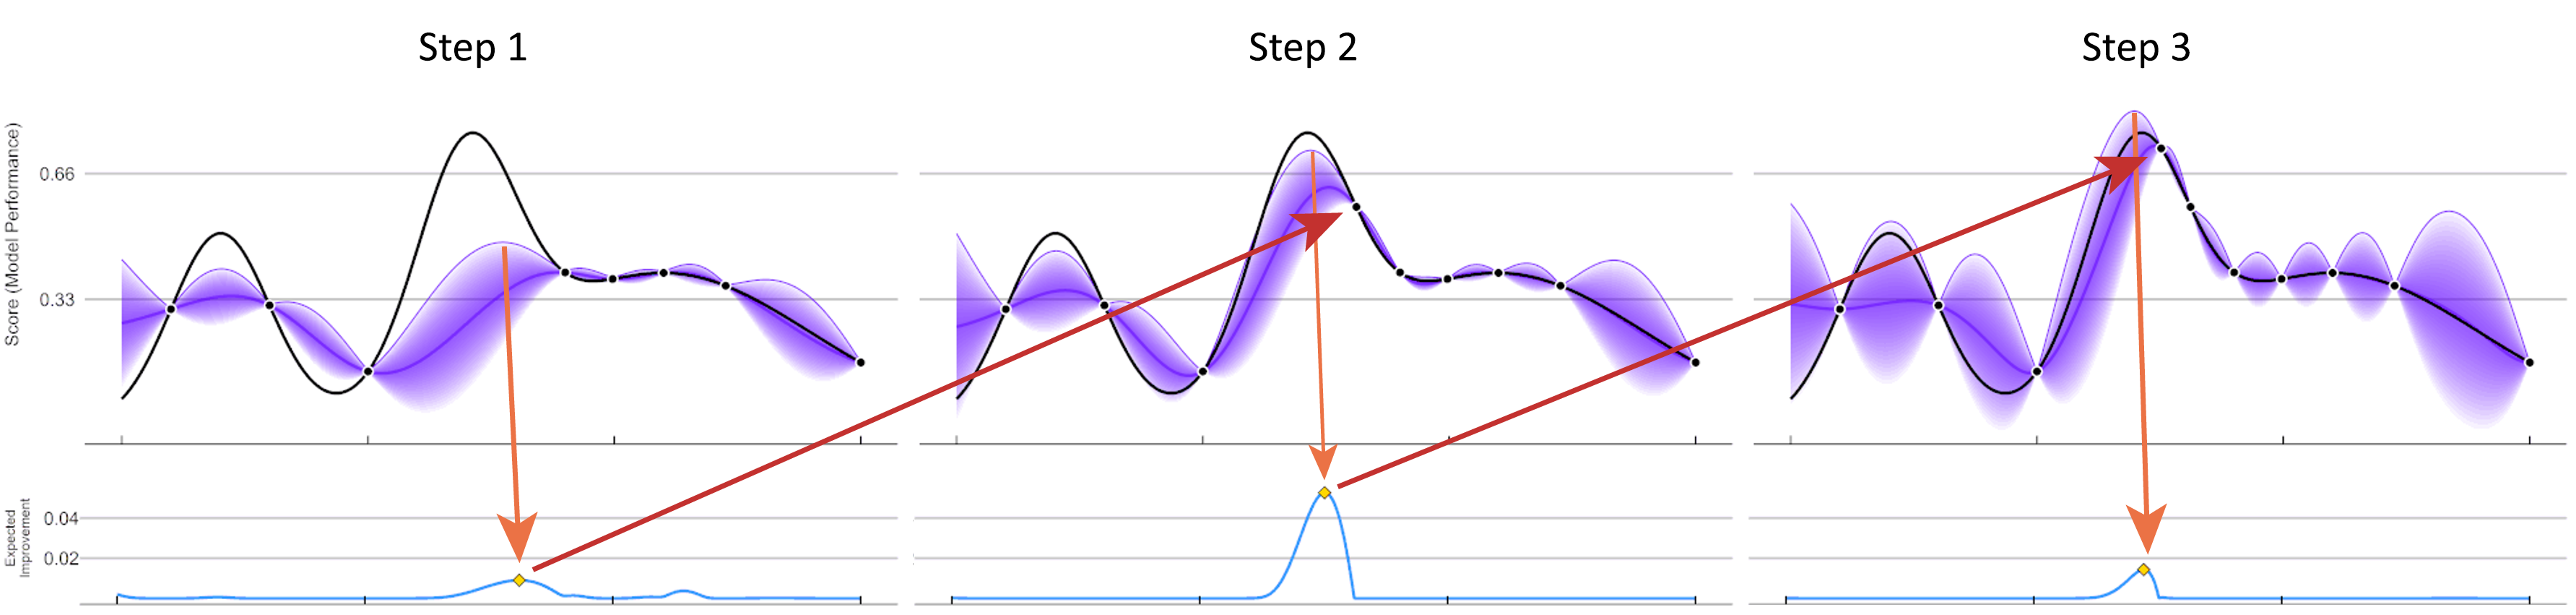
\includegraphics[width=1.0\textwidth]{img/bayesian_opt.png}
 \caption{Schematic illustration of Bayesian optimization. The to-be-optimized function is shown in black, the Gaussian uncertainty in the purple bands, and the surrogate model is the blue function below. CC BY-SA 4.0 AnotherSamWilson on Wikimedia Commons.}
 \label{fig:bayesian_opt}
\end{figure}

In \autoref{fig:bayesian_opt}, a schematic representation of the process of Bayesian optimization can be seen. Firstly, a few arbitrary points are sampled on the function. This is done in order to be able to fit a Gaussian probability estimation to the function using the process of kriging. This results in the situation shown in \textit{step 1} in the figure. From the probability estimation, the surrogate model (shown at the bottom) is then determined. The algorithm samples the point which optimizes the surrogate model, and uses it to obtain a new proability estimation, \textit{step 2}. At step 2, the process is repeated, leading to step 3. It can be seen that at this point, the estimation is already close to the global optimum. \\

In practice this model will be more complex than the one-dimensional function shown in \autoref{fig:bayesian_opt}, and therefore will require more evaluations to reach the optimum. This becomes especially apparent as the dimensionality of the problem increases: as the sparseness of the solution space increases, fitting a meaningful Gaussian probability estimate naturally becomes more difficult (\cite{Bayesian}). A bigger problem, however, is the presence of noise in the function. Due to the random selection of asteroids and the probabilistic nature of the detection model, some noise is to be expected in the results. During the optimization process, care will have to be taken to ensure that the optimizer does not attempt to exploit the noise in the function, as this will lead to an overfit (\cite{Surrogate}). \\

\begin{figure}[htbp]
 \centering
 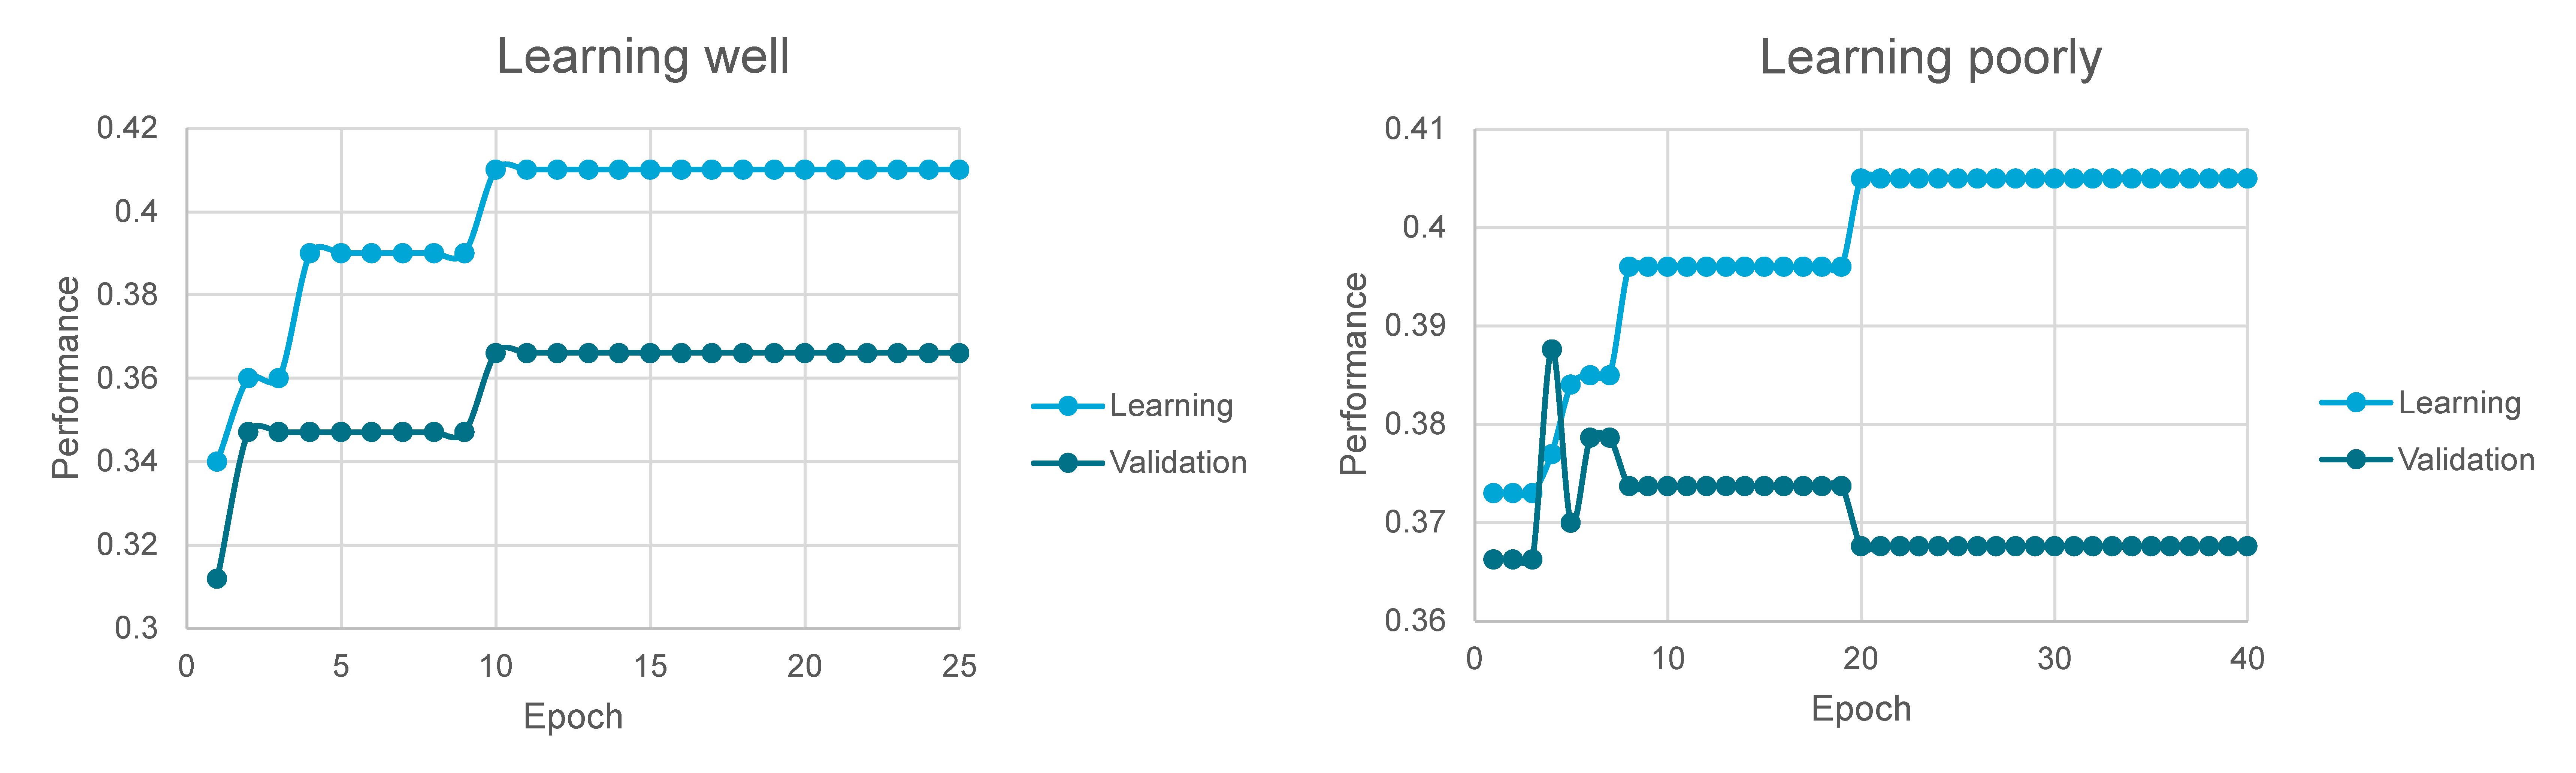
\includegraphics[width=1.0\textwidth]{img/validation_example.pdf}
 \caption{Example of a system which learns well, and a system which learns poorly, overfitting instead. Note: epoch here refers to the step in the learning process, not the datum of an astronomical coordinate system.}
 \label{fig:validation_example}
\end{figure}

Such \textit{overfit} can be examined by performing a validation calculation at set points during the optimization process. This will provide two sets of survey performance values: the \textit{learning} value, which is the performance predicted by the optimizer, and the \textit{validation} value, which is the performance obtained by evaluating the solution found by the optimizer against an independent dataset. In case the optimizer is learning well, an increase in learning performance will also result in an increase in validation performance. This implies the optimizer has found a feature which is actually relevant to the model performance (\cite{DeepLearning}). Alternatively, if the learning performance increases, but the validation performance either stays constant, or even decreases, it means the system is overfitting: the optimizer is attempting to exploit the noise in the signal. An example of this can be seen in \autoref{fig:validation_example}. (see \cite{DeepLearning}, chapter 7 and 8 for a more thorough discussion on learning, validation, and overfitting)\\


In the case of severe overfitting, such as might occur when a highly dimensional solution is required, a backup method is to use a method based on a random search. This method is very simple: throughout the entire solution space, random points are uniformly sampled. Then, after a sufficient number of iterations, this process is repeated on a smaller space around the found optimum (this starts a new optimization cycle, essentially ``resetting'' the overfit), to find a more precise optimum. This can then be repeated a number of times to obtain the global optimum. Although slow and seamingly unelegant, this method has the benefit that it is largely independent of the function itself, and therefore is not prone to overfitting or getting stuck in a local minimum (see \cite{HOML} for a thorough discription, as well as discourse on why this method is preferable to a grid search).

\section{Research Process}
\label{sec:methodologyprocess}
The final consideration in terms of methodology is the actual research process. After implementation of the above, it might be simple to leave the simulation to the optimizer and see what ``optimal'' solutions results. However, this would not be a prudent course of action. Not only would the survey simulation function as a black box, making it hard to ascertain whether or not the optimizer yields useful results, such an approach would also not provide meaningful insight into the behavior of various parts of the system apart from the optimum itself. Therefore, a more complex research process was set up. The goal of this process is to gain insight into the behavior of individual elements of the solution next to finding the optimal solutions to the problem. Not only will this help in interpreting the results of the optimization, it will also provide a frame of reference for judging the quality of the optimization results to alleviate inherent problems such as noise and overfitting.\\

The process works up from simple solutions to more complex solutions, evaluating the outcomes at every step. This is mainly related to how much freedom the solution of the system has. However before discussing this, it is important to first establish the position of the number of spacecraft and their payload in this process. With regards to the number of spacecraft, the optimization problem is not very useful: assuming the optimizer functions correctly, an increase in the number of spacecraft will always yield an improvement in the survey completeness, or at worst no change at all. Therefore, as far as survey completeness is concerned, there is logically no \textit{optimal} number of spacecraft. On the contrary, discovering the effect of increasing or decreasing the number of spacecraft in the system is one of the most important goals of the research project. Therefore, the number of spacecraft is treated mostly as a parameter outside of the optimization process, and solutions are tested for a large range of system sizes. The optimizer is thus used as a tool to evaluate the best performance which might be expected from a certain number of spacecraft, and how this changes as the number of spacecraft changes. The spacecraft's payload composition is subject to a similar treatment: although the performance of the systems is dependent on current hardware capabilities, this might change in the future. Therefore, it is interesting to examine the behavior of not only the optimal payload configuration, but also, in more limited fashion, all payload compositions. To complement this, research will be done into the effects of the payload on the performance, and how layouts combining different payloads function.\\

After that distinction, the general research process can be laid out. Firstly, the simulation was extensively verified, as mentioned throughout this section. In addition, where relevant, validation is performed to ensure that results translate to actual applications of the system, and to allow for accurate comparison to other survey proposals. As the validation requires interpretation of the results, it is discussed further after the results, in \autoref{ch:vandv}. Then, as the quality of the simulation has been established, the following research steps are carried out:
\begin{enumerate}
 \item Through a grid search methodology, all 1-to-1 relations between variables and survey completeness are examined. Although this will not provide very detailed results, it will provide insight into the influence of various parameters. Next to being useful knowledge in and of itself, this will also provide a framework to judge the performance of the optimizer later.
 \item Using knowledge from the first step, preliminary optimization is carried out to determine a useful range of number of spacecraft for which to carry out more detailed analysis.
 \item For this range of number of spacecraft, simple optimizations in which the spacecraft are all in the same orbit (thus limiting the parameter space) is carried out to provide an initial assessment of performance. This process is repeated for different payload compositions to determine the useful payload compositions to continue the analysis with.
 \item In parallel, for both visual light and thermal infrared systems, optimization is performed of systems in which all spacecraft are in the same orbit, with only a different anomaly at epoch.
 \item Continuing with an optimal range of spacecraft number and payload composition, parameters are increasingly freed up to the optimizer, first allowing for different circular orbits per spacecraft, and later also adding eccentricity. Due to time constraints, inclination (and therefore right ascension) and argument of periapsis are left for future research. At this stage, a thorough analysis of the optimizer will have to be performed to assess whether the results are valid or the optimizer is starting to overfit.
 \item As the complexity increases, the global optimal solutions to the problem are found, and it can be determined how the performance relates to other survey proposals.
 \item Lastly, the optimization effort is continued to higher numbers of spacecraft to obtain knowledge on how many asteroids can feasibly be detected. This will finalize the research effort by providing a framework for mission designers to base their initial sizing of the system on.
\end{enumerate}
It is expected that the research goals, as formulated in \autoref{sec:researchquestions} will be adequately answered through this process.
